\clearpage
\section{On-chain Protocol}\label{sec:on-chain}
% FIXME: update all figures: removed n and decrement changes
\todo{Update figures}

\todo{Open problem: ensure abort is always possible. e.g. by individual aborts or undoing commits}
\todo{Open problem: ensure fanout is always possible, e.g. by limiting complexity of $U_0$}

The following sections describe the the \emph{on-chain} protocol controlling the
life-cycle of a Hydra head, which can be intuitively described as a state
machine (see Figure~\ref{fig:SM_states_basic}). Each transition in this state
machine is represented and caused by a corresponding Hydra protocol transaction
on-chain: $\mtxInit{}$, $\mtxCom{}$, $\mtxAbort{}$, $\mtxCollect{}$,
$\mtxDecrement{}$, $\mtxClose{}$, $\mtxContest{}$, and $\mtxFanout{}$.

% TODO: Could include a combined overview, slightly more detailed than Figure 1
% of the transaction trace for the full life cycle maybe?

\noindent The protocol defines one minting policy script and three validator scripts:
\begin{itemize}
	\item $\muHead$ governs minting of state and participation tokens in
	      $\mtxInit{}$ and burning of these tokens in $\mtxAbort{}$ and
	      $\mtxFanout{}$.
	\item $\nuInitial$ controls how UTxOs are committed to the head in
	      $\mtxCommit{}$ or when the head initialiazation is aborted via
	      $\mtxAbort{}$.
	\item $\nuCommit$ controls the collection of committed UTxOs into the head in
	      $\mtxCollect$ or that funds are reimbursed in an $\mtxAbort{}$.
	\item $\nuHead$ represents the main protocol state machine logic and ensures
	      contract continuity throughout $\mtxCollect{}$, $\mtxDecrement{}$,
	      $\mtxClose{}$, $\mtxContest{}$ and $\mtxFanout{}$.
\end{itemize}

\subsection{Init transaction}\label{sec:init-tx}

The \mtxInit{} transaction creates a head instance and establishes the initial
state of the protocol and is shown in Figure~\ref{fig:initTx}. The head
instance is represented by the unique currency identifier $\cid$ created by
minting tokens using the $\muHead$ minting policy script which is parameterized
by a single output reference parameter $\seed \in \tyOutRef$:
\[
	\cid = \hash(\muHead(\seed))
\]

\begin{figure}
	\centering
	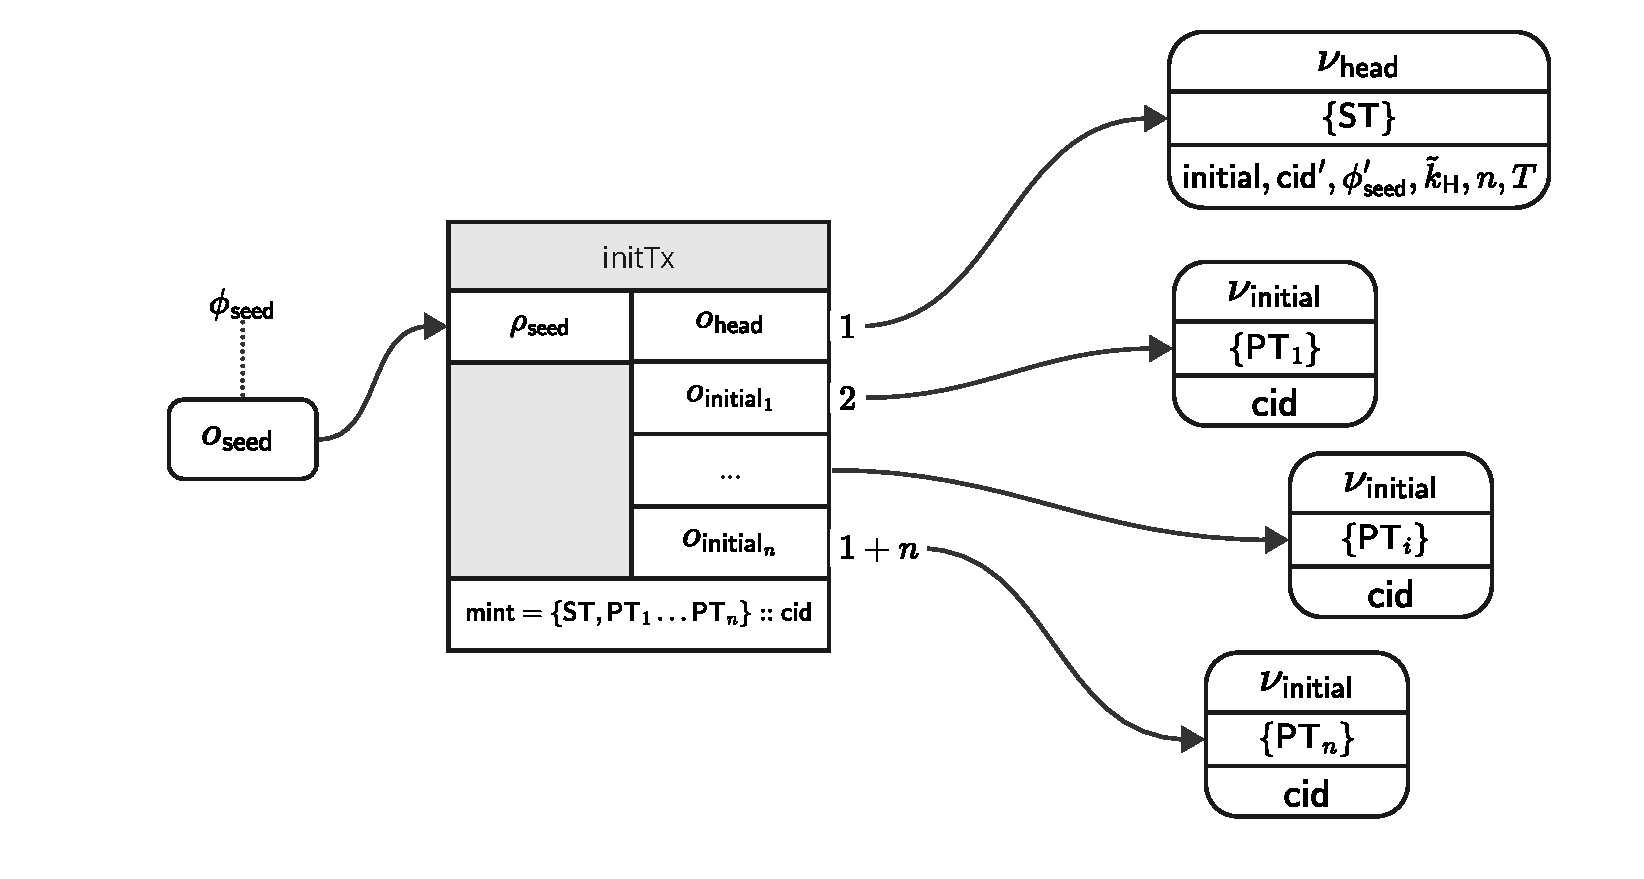
\includegraphics[width=0.8\textwidth]{figures/initTx.pdf}
	\caption{\mtxInit{} transaction spending a seed UTxO, and producing the head
		output in state $\stInitial$ and initial outputs for each participant.}\label{fig:initTx}
\end{figure}

\noindent Two kinds of tokens are minted:
\begin{itemize}
	\item A single \emph{State Thread (ST)} token marking the head output. This
	      output contains the state of the protocol on-chain and the token ensures
	      contract continuity. The token name is the well known string
	      \texttt{HydraHeadV1}, i.e.
	      $\st = \{\cid \mapsto \texttt{HydraHeadV1} \mapsto 1\}$.
	\item One \emph{Participation Token (PT)} per participant
	      $i \in \{1 \dots |\hydraKeys|  \}$ to be used for authenticating further
	      transactions and to ensure every participant can commit and cannot be
	      censored. The token name is the participant's verification key hash
	      $\keyHash_{i} = \hash(\msVK_{i})$ of the verification key as received
	      during protocol setup, i.e.
	      $\pt_{i} = \{\cid \mapsto \keyHash_{i} \mapsto 1\}$.
\end{itemize}

\noindent Consequently, the \mtxInit{} transaction
\begin{itemize}
	\item has at least input $\seed$,
	\item mints the state thread token $\st$, and one $\pt$ for each of the $|\hydraKeys|$
	      participants with policy $\cid$,
	\item has $|\hydraKeys|$ initial outputs $o_{\mathsf{initial}_{i}}$ with datum $\datumInitial{} = \cid$,
	\item has one head output
	      $o_{\mathsf{head}}$, which captures
	      the initial state of the protocol in the datum
	      \[
		      \datumHead = (\stInitial,\cid',\seed',\hydraKeys,\cPer)
	      \]
	      where
	      \begin{mitemize}
		      \item $\stInitial$ is a state identifier,
		      \item $\cid'$ is the unique currency id of this instance,
		      \item $\seed'$ is the output reference parameter of $\muHead$,
		      \item $\hydraKeys$ are the off-chain multi-signature keys from the setup
		      phase,
		      \item $\cPer$ is the contestation period.
	      \end{mitemize}
\end{itemize}

\noindent The $\muHead(\seed)$ minting policy is the only script that verifies
init transactions and can be redeemed with either a $\mathsf{mint}$ or
$\mathsf{burn}$ redeemer:
% TODO: mint redeemer conflicts with mint field
\begin{itemize}
	\item When evaluated with the $\mathsf{mint}$ redeemer,
	      \begin{menumerate}
		      \item The seed output is spent in this transaction. This guarantees uniqueness of the policy $\cid$ because the EUTxO ledger ensures that $\seed$ cannot be spent twice in the same chain.
		      $(\seed, \cdot) \in \txInputs$
		      \item All entries of $\txMint$ are of this policy and of single quantity $\forall \{c \mapsto \cdot \mapsto q\} \in \txMint : c = \cid \land q = 1$
		      \item Right number of tokens are minted $|\txMint| = |\hydraKeys| + 1$
		      % TODO: |\txMint| may not be clear to the reader, maybe combine with item above, but be more explicit.
		      \item State token is sent to the head validator $\st \in \valHead$ % TODO: fact that it is goverend by nuHead is a bit implicit here.
		      \item \textcolor{blue}{The correct number of initial outputs are present $|(\cdot, \nuInitial, \cdot) \in \txOutputs| = |\hydraKeys|$}
		      % XXX: this is implied by the ledger, so can be removed
		      \item All participation tokens are sent to the initial validator as an initial output $\forall i \in [1 \dots |\hydraKeys|] : \{\cid \mapsto \cdot \mapsto 1\} \in \valInitial{i}$
		      \item The $\datum_{\mathsf{head}}$ contains own currency id $\cid = \cid'$ and the right seed reference $\seed = \seed'$
		      \item All initial outputs have a $\cid$ as their datum: $\forall i \in [1 \dots |\hydraKeys|] : \cid = \datumInitial{i}$
	      \end{menumerate}
	\item When evaluated with the $\mathsf{burn}$ redeemer,
	      \begin{menumerate}
		      \item All tokens for this policy in $\txMint$ need to be of negative quantity
		      $\forall \{\cid \mapsto \cdot \mapsto q\} \in \txMint : q < 0$.
	      \end{menumerate}
\end{itemize}

\noindent \textbf{Important:} The $\muHead$ minting policy only ensures
uniqueness of $\cid$, that the right amount of tokens have been minted and sent
to $\nuHead$ and $\nuInitial$ respectively, while these validators in turn
ensure continuity of the contract. However, it is \textbf{crucial} that all head
members check that head output always contains an $\st$ token of policy $\cid$
which satisfies $\cid = \hash(\muHead(\seed))$. The $\seed$ from a head datum
can be used to determine this. Also, head members should verify whether the
correct verification key hashes are used in the $\pt$s and the initial state is
consistent with parameters agreed during setup. See the initialTx behavior in
Figure~\ref{fig:off-chain-prot} for details about these checks.\\

\subsection{Commit Transaction}\label{sec:commit-tx}

A \mtxCom{} transaction may be submitted by each participant
$\forall i \in \{1 \dots |\hydraKeys|\}$ to commit some UTxO into the head or
acknowledge to not commit anything. The transaction is depicted in
Figure~\ref{fig:commitTx} and has the following structure:
\begin{itemize}
	\item One input spending from $\nuInitial$ with datum $\datumInitial{}$,
	      where value $\valInitial{i}$ holds a $\pt_i$, and the redeemer
	      $\redeemerInitial{} \in \tyOutRef^{*}$ is a list of output
	      references to be committed,
	\item zero or more inputs with reference $\txOutRef_{\mathsf{committed}_{j}}$
	      spending output $o_{\mathsf{committed}_{j}}$ with
	      $\val_{\mathsf{committed}_{j}}$,
	\item one output paying to $\nuCommit$ with value $\valCommit{i}$ and datum $\datumCommit{}$.
\end{itemize}

\noindent The $\nuInitial$ validator with $\datumInitial{} = \cid$ and
$\redeemerInitial{} = \underline{\txOutRef}_{\mathsf{committed}}$ ensures that:
\begin{menumerate}
	\item All committed value is in the output
	$\valCommit{i} \supseteq \valInitial{i} \cup (\bigcup_{j=1}^{m} \val_{\mathsf{committed}_{j}})$
	\footnote{The $\supseteq$ is important for real world situations where the values
		might not be exactly equal due to ledger constraints (i.e. to ensure a
		minimum value on outputs).}
	\item Currency id and committed outputs are recorded in the output datum
	$\datumCommit{} = (\cid, C_{i})$, where
	$C_{i} = \forall j \in \{1 \dots m\} : [(\txOutRef_{\mathsf{committed}_{j}},\bytes(o_{\mathsf{committed}_{j}}))]$
	is a list of all committed UTxO recorded as tuples on-chain.
	\item Transaction is signed by the right participant
	$\exists \{\cid \mapsto \keyHash_{i} \mapsto 1\} \in \valInitial{} \Rightarrow \keyHash_{i} \in \txKeys$
	\item No minting or burning $\txMint = \varnothing$
\end{menumerate}

\noindent The $\nuCommit$ validator ensures the output is collected by either a
\mtxCCom{} in Section~\ref{sec:collect-tx} or \mtxAbort{} in
Section~\ref{sec:abort-tx} transaction of the on-chain state machine, selected
by the appropriate redeemer.

\begin{figure}
	\centering
	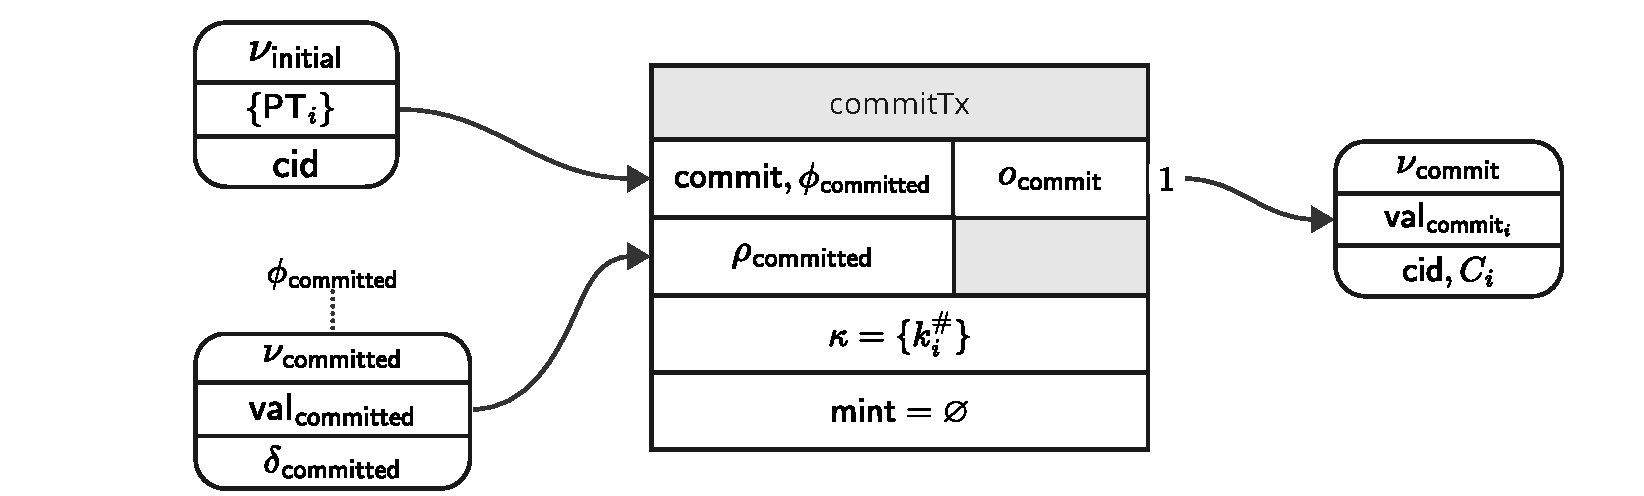
\includegraphics[width=0.8\textwidth]{figures/commitTx.pdf}
	\caption{\mtxCom{} transaction spending an initial output and a single
		committed output, and producing a commit output.}\label{fig:commitTx}
\end{figure}
\todo{update with multiple commits}

\subsection{Abort Transaction}\label{sec:abort-tx}

The \mtxAbort{} transaction (see Figure~\ref{fig:abortTx}) allows a
party to abort the creation of a head and consists of
\begin{itemize}
	\item one input spending from $\nuHead$ holding the $\st$ with $\datumHead$,
	\item $\forall i \in \{1 \dots |\hydraKeys|\}$ inputs either
	      \begin{itemize}
		      \item spending from $\nuInitial$ with with $\pt_{i} \in \valInitial{i}$ and $\datumInitial{i} = \cid$, or
		      \item spending from $\nuCommit$ with with $\pt_{i} \in \valCommit{i}$ and $\datumCommit{i} = (\cid, C_{i})$,
	      \end{itemize}
	\item outputs $o_{1} \dots o_{m}$ to redistribute already committed UTxOs.
\end{itemize}

Note that \mtxAbort{} represents a final transition of the state
machine and hence there is no state machine output.

\noindent Each spent $\nuInitial$ validator with $\datumInitial{i} = \cid$ and $\redeemerInitial{i} = \mathsf{abort}$ ensures that:
\begin{menumerate}
	\item The state token of currency $\cid$ is getting burned $\{\st \mapsto -1\} \subseteq \txMint$.
\end{menumerate}

\noindent Each spent $\nuCommit$ validator with $\datumCommit{i} = (\cid,\cdot)$ and $\redeemerCommit{i} = \mathsf{abort}$ ensures that:
\begin{menumerate}
	\item The state token of currency $\cid$ is getting burned $\{\st \mapsto -1\} \subseteq \txMint$.
\end{menumerate}

\noindent The $\muHead(\seed)$ minting policy governs the burning of tokens via
redeemer $\mathsf{burn}$ that:
\begin{menumerate}
	\item All tokens in $\txMint$ need to be of negative quantity
	$\forall \{\cid \mapsto \cdot \mapsto q\} \in \txMint : q < 0$.
\end{menumerate}

\noindent The state-machine validator $\nuHead$ is spent with
$\redeemerHead = (\mathsf{abort}, m)$, where $m$ is the number of outputs to
reimburse, and checks:
\begin{menumerate}
	\item State is advanced from $\datumHead \sim \stInitial$ to terminal state
	$\stFinal$:
	\[
		(\stInitial,\cid,\seed,\hydraKeys,\cPer) \xrightarrow[m]{\stAbort} \stFinal.
	\]
	\item All UTxOs committed into the head are reimbursed exactly as they were
	committed. This is done by comparing hashes of serialised representations of
	the $m$ reimbursing outputs $o_{1} \dots o_{m}$\footnote{Only the first $m$
		outputs are used for reimbursing, while more outputs may be present in the
		transaction, e.g for returning change.} with the canonically combined
	committed UTxOs in $C_{i}$:
	\[
		\hash(\bigoplus_{j=1}^{m} \bytes(o_{j})) = \combine([C_{i} ~ | ~ \forall [1 \dots |\hydraKeys|], C_{i} \neq \bot])
	\]

	\item Transaction is signed by a participant $\exists \{\cid \mapsto \keyHash_{i} \mapsto -1\} \in \txMint \Rightarrow \keyHash_{i} \in \txKeys$.
	\item All tokens are burnt
	$|\{\cid \mapsto \cdot \mapsto -1\} \in \txMint| = |\hydraKeys| + 1$.
\end{menumerate}

\begin{figure}
	\centering
	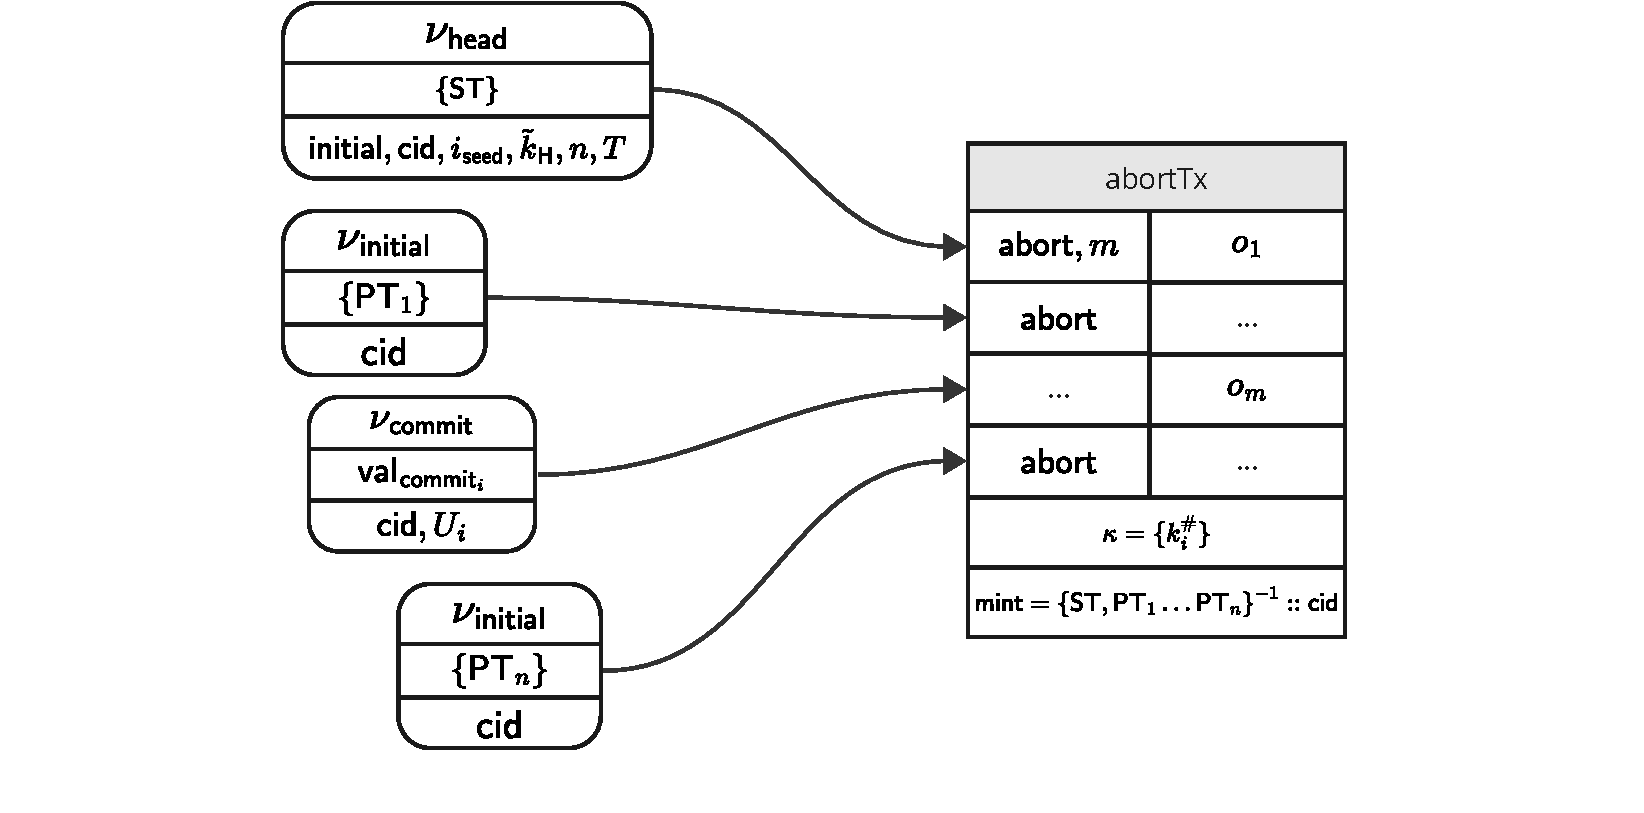
\includegraphics[width=0.8\textwidth]{figures/abortTx.pdf}
	\caption{\mtxAbort{} transaction spending the $\stInitial$ state head
		output and collecting all initial and commit outputs, which get reimbursed
		by outputs $o_{1} \dots o_{m}$. Note that each $\pt$ may be in either, an
		initial or commit output.}\label{fig:abortTx}
\end{figure}

\subsection{CollectCom Transaction}\label{sec:collect-tx}

\noindent The \mtxCCom{} transaction (Figure~\ref{fig:collectComTx}) collects
all the committed UTxOs to the same head. It has
\begin{itemize}
	\item one input spending from $\nuHead$ holding the $\st$ with $\datumHead$,
	\item $\forall i \in \{1 \dots |\hydraKeys|\}$ inputs spending commit outputs
	      $(\valCommit{i}, \nuCommit, \datumCommit{i})$ with $\pt_{i} \in \valCommit{i}$
	      and $\datumCommit{i} = (\cid, C_{i})$, and
	\item one output paying to $\nuHead$ with value $\valHead'$ and
	      datum $\datumHead'$.
\end{itemize}

\noindent The state-machine validator $\nuHead$ is spent with
$\redeemerHead = \mathsf{collect}$ and checks:
\begin{menumerate}
	\item State is advanced from $\datumHead \sim \stInitial$ to
	$\datumHead' \sim \stOpen$, parameters $\cid,\hydraKeys,\cPer$ stay
	unchanged and the new state is governed again by $\nuHead$
	\[
		(\stInitial,\cid,\seed,\hydraKeys,\cPer) \xrightarrow{\stCollect} (\stOpen,\cid,\hydraKeys,\cPer,v,\eta)
	\]
	where snapshot version is initialized as $v = 0$.
	\item Commits are collected in $\eta$
	\[
		\eta = U^{\#} = \combine([C_{1}, \dots, C_{n}])
	\]
	where $n = |\hydraKeys|$ and
	\[
		\combine(\underline{C}) = \hash(\mathsf{concat}({\sortOn(1, \mathsf{concat}(\underline{C}))}^{\downarrow2}))
	\]
	That is, given a list of committed UTxO $\underline{C}$, where each element is
	a list of output references and the serialised representation of what was
	committed, $\combine$ first concatenates all commits together, sorts this list
	by the output references, concatenates all bytes and hashes the
	result\footnote{Sorting is required to ensure a canonical representation which
		can also be reproduced from the UTxO set later in the fanout.}.

	\item All committed value captured and no value is extracted
	\[
		\valHead' = \valHead \cup (\bigcup_{i=1}^{n} \valCommit{i})
	\]
	\item Every participant had the chance to commit, by checking all tokens are
	present in output\footnote{This is sufficient as a Head participant would
		check off-chain whether a Head is initialized correctly with the right
		number of tokens.}
	% NOTE: Implemented slightly different as we would only count PTs and = n
	\[
		|\{\cid \rightarrow . \rightarrow 1\} \in \valHead'| = |\hydraKeys| + 1
	\]
	\item Transaction is signed by a participant
	\[
		\exists \{\cid \mapsto \keyHash_{i} \mapsto 1\} \in \valCommit{i} \Rightarrow \keyHash_{i} \in \txKeys
	\]
	\item No minting or burning
	\[
		\txMint = \varnothing
	\]
\end{menumerate}

\noindent Each spent $\nuCommit$ validator with $\datumCommit{i} = (\cid,\cdot)$ and $\redeemerCommit{i} = \mathsf{collect}$ ensures that:
\begin{menumerate}
	\item The state token of currency $\cid$ is present in the output value
	\[
		\st \in \valHead'
	\]
\end{menumerate}

\begin{figure}
	\centering
	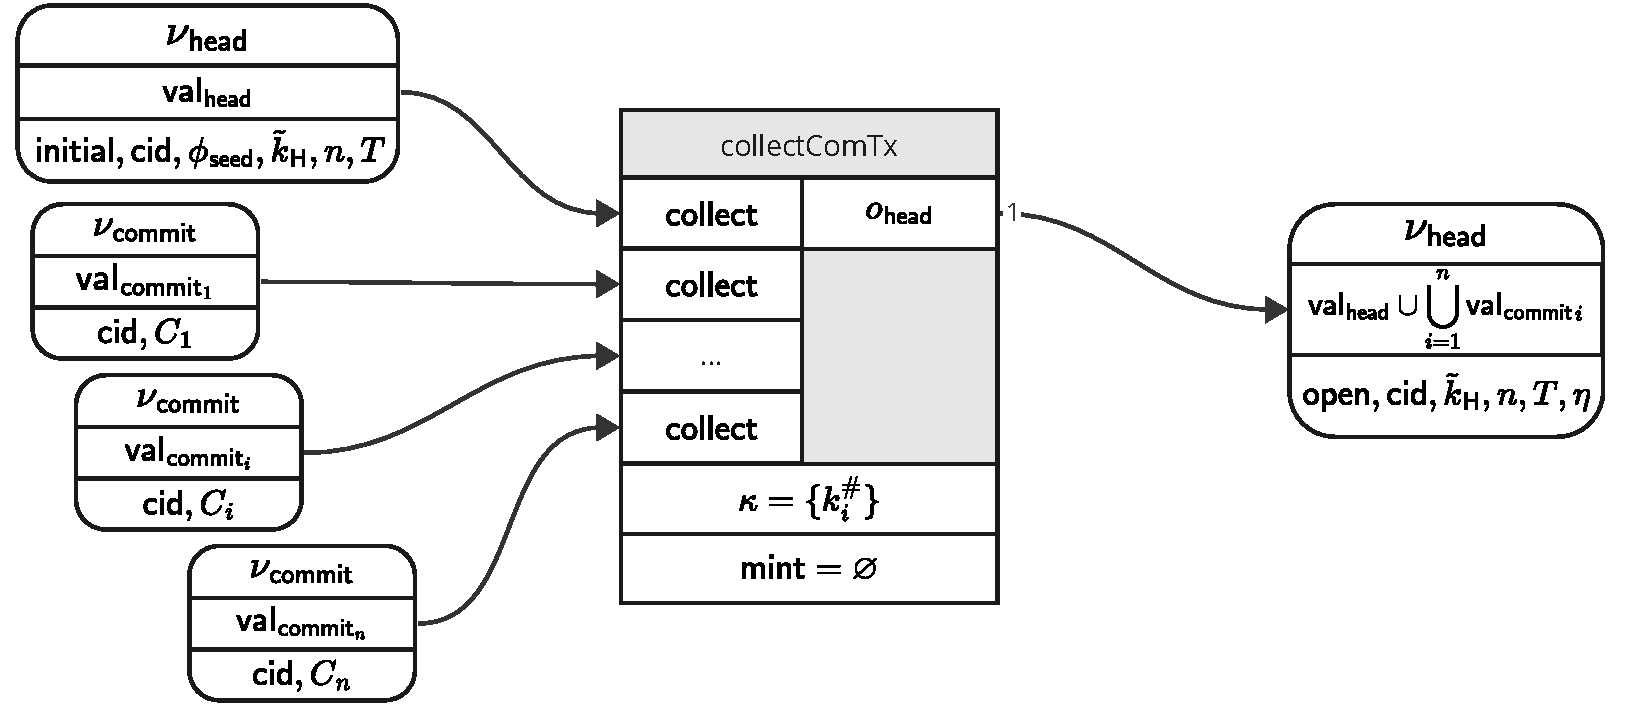
\includegraphics[width=0.8\textwidth]{figures/collectComTx.pdf}
	\caption{\mtxCCom{} transaction spending the head output in $\stInitial$
		state and collecting from multiple commit outputs into a single
		$\stOpen$ head output.}\label{fig:collectComTx}
\end{figure}

\subsection{Decrement Transaction}\label{sec:decrement-tx}

\noindent The \mtxDecrement{} transaction (Figure~\ref{fig:DecrementTx}) allows
a party to remove a UTxO from an already open head and consists of:

\begin{itemize}
	\item one input spending from $\nuHead$ holding the $\st$ with $\datumHead$,
	\item one output paying to $\nuHead$ with value $\valHead'$ and
	      datum $\datumHead'$,
	\item one or more decommit outputs $o_{2} \dots o_{m+1}$.
\end{itemize}

\noindent The state-machine validator $\nuHead$ is spent with
$\redeemerHead = (\mathsf{decrement}, \xi, s, m)$, where $\xi$ is a multi-signature of
the decrement snapshot which authorizes removal of some UTxO, $s$ is the
used snapshot number and $m$ is the number of outputs to distribute. The
validator checks:
\begin{menumerate}
	\item State is advanced from $\datumHead \sim \stOpen$ to
	$\datumHead' \sim \stOpen$, parameters $\cid,\hydraKeys,\cPer$ stay
	unchanged and the new state is governed again by $\nuHead$
	\[
		(\stOpen,\cid,\hydraKeys,\cPer,v,\eta) \xrightarrow[\xi, s, m]{\mathsf{decrement}} (\stOpen,\cid,\hydraKeys,\cPer,v',\eta')
	\]
	\item New version $v'$ is incremented correctly
	\[
		v' = v + 1
	\]
	\item $\xi$ is a valid multi-signature of the currency id $\cid$, the current state version $v$, and the new state $\eta'$
	\[
		\msVfy(\hydraKeys,(\cid || v || s || \eta' || \eta_{\omega}),\xi) = \true
	\]
	where snapshot number $s$ is provided through the redeemer and $\eta_{\omega}$ must be the digest of all removed UTxO
	\[
		\eta_{\omega} = U^{\#}_{\omega}  = \hash(\bigoplus_{j=2}^{m+1} \bytes(o_{j}))
	\]
	\item The value in the head output is decreased accordingly
	\todo{Redundant to above? Only check $\valHead' < \valHead$?}
	\[
		\valHead' \cup (\bigcup_{j=2}^{m+1} \val_{o_{j}}) = \valHead
	\]
	\item Transaction is signed by a participant
	\todo{Allow anyone to do decrements?}
	\[
		\exists \{\cid \mapsto \keyHash_{i} \mapsto 1\} \in \valHead' \Rightarrow \keyHash_{i} \in \txKeys
	\]
\end{menumerate}

\begin{figure}
	\centering
	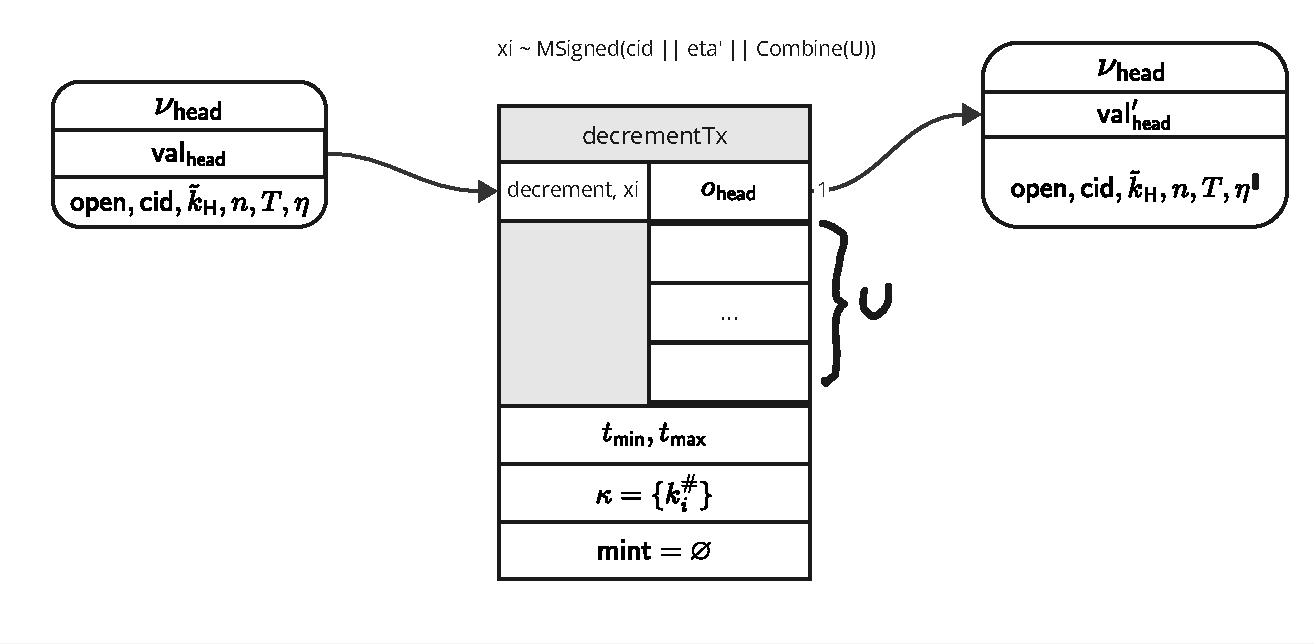
\includegraphics[width=0.8\textwidth]{figures/decrementTx.pdf}
	\caption{\mtxDecrement{} transaction spending an open head output,
		producing a new head output and multiple decommitted outputs.}\label{fig:decrementTx}
\end{figure}

\subsection{Close Transaction}\label{sec:close-tx}

In order to close a head, a head member may post the \mtxClose{} transaction
(see Figure~\ref{fig:closeTx}). This transaction has
\begin{itemize}
	\item one input spending from $\nuHead$ holding the $\st$ with $\datumHead$,
	\item one output paying to $\nuHead$ with value $\valHead'$ and
	      datum $\datumHead'$.
\end{itemize}

\begin{figure}
	\centering
	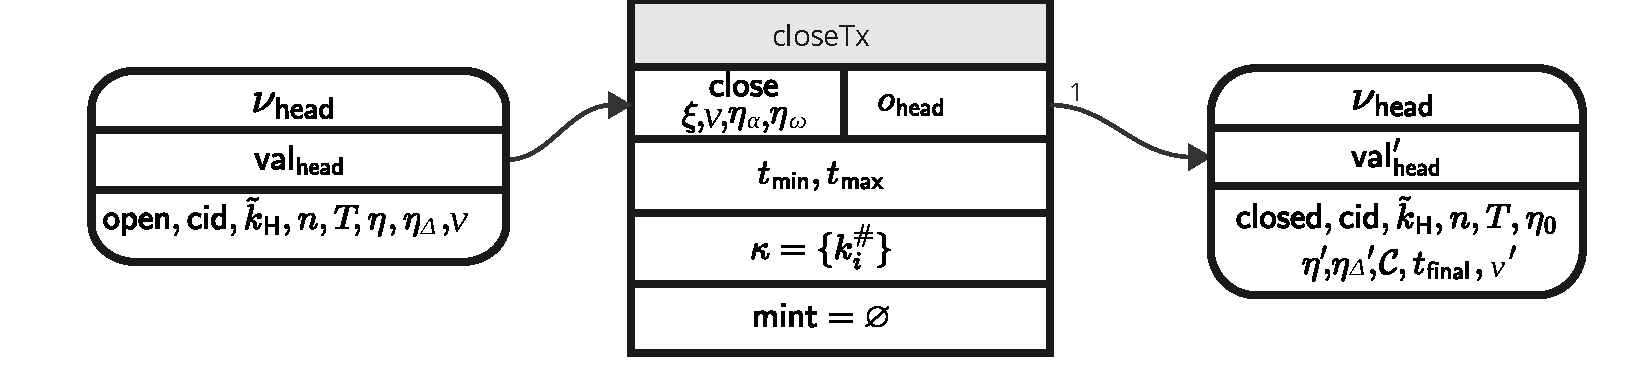
\includegraphics[width=0.8\textwidth]{figures/closeTx.pdf}
	\caption{\mtxClose{} transaction spending the $\stOpen$ head output and producing a $\stClosed$ head output.}\label{fig:closeTx}
\end{figure}

\noindent The state-machine validator $\nuHead$ is spent with
$\redeemerHead = (\mathsf{close}, \mathsf{CloseType})$, where
$\mathsf{CloseType}$ is a hint against which open state to close and checks:
\begin{menumerate}
	\item State is advanced from $\datumHead \sim \stOpen$ to
	$\datumHead' \sim \stClosed$, parameters $\cid,\hydraKeys,\cPer$
	stay unchanged and the new state is governed again by $\nuHead$
	\[
		(\stOpen,\cid,\hydraKeys,\cPer,v,\eta) \xrightarrow[\mathsf{CloseType}]{\stClose} (\stClosed,\cid,\hydraKeys,\cPer,v',s',\eta',\eta_{\Delta}',\contesters,\Tfinal)
	\]

	\item Last known open state version is recorded in closed state
	\[
		v' = v
	\]

	\item Based on the redeemer $\mathsf{CloseType} = \mathsf{Initial} \cup (\mathsf{Unused}, \xi) \cup (\mathsf{Used}, \xi,  \eta_{\omega})$, where $\xi$ is a multi-signature of the closing snapshot and $\eta_{\omega}$ is a digest of the UTxO to decommit, three cases are distinguished:
	\begin{menumerate}
		\item $\mathsf{Initial}$: The initial snapshot is used to close the head and open state was not updated. No signatures are available and it suffices to check
		\[
			v = 0
		\]
		\[
			s' = 0
		\]
		\[
			\eta' = \eta
		\]
		\item $\mathsf{Unused}$: Closing snapshot refers to current state version $v$ and any UTxO to decommit need to be present in the closed state too.
		\[
			\msVfy(\hydraKeys,(\cid || v || s' || \eta' || \eta_{\Delta}'),\xi) = \true
		\]
		which implies $\eta_{\Delta}' = \eta_{\omega}$ while $\eta_{\omega}$ does not need to be provided.
		\item $\mathsf{Used}$: Closing snapshot refers the previous state $v - 1$ and any UTxO to decommit of the closing snapshot must not be recorded in the closed state.
		\[
			\eta_{\Delta}' = \bot
		\]
		\[
			\msVfy(\hydraKeys,(\cid || v - 1 || s' || \eta' || \eta_{\omega}),\xi) = \true
		\]
		where $\eta_{\omega}$ is provided by the redeemer\footnote{$\eta_{\omega}$ needs to be provided to verify the signature, but is otherwise not relevant for the closed state}.
	\end{menumerate}
	% TODO: detailed CDDL definition of msg

	\item Initializes the set of contesters
	\[
		\contesters = \emptyset
	\]
	This allows the closing party to also contest and is required for use
	cases where pre-signed, valid in the future, close transactions are
	used to delegate head closing.

	\item Correct contestation deadline is set
	\[
		\Tfinal = \txValidityMax + T
	\]
	\item Transaction validity range is bounded by
	\[
		\txValidityMax - \txValidityMin \leq T
	\]
	to ensure the contestation deadline $\Tfinal$ is at most $2*T$ in the future.
	\item Value in the head is preserved
	\[
		\valHead' = \valHead
	\]
	\item Transaction is signed by a participant
	\[
		\exists \{\cid \mapsto \keyHash_{i} \mapsto 1\} \in \valCommit{i} \Rightarrow \keyHash_{i} \in \txKeys
	\]
	\item No minting or burning
	\[
		\txMint = \varnothing
	\]
\end{menumerate}

\subsection{Contest Transaction}\label{sec:contest-tx}

The \mtxContest{} transaction (see Figure~\ref{fig:contestTx}) is posted by a
party to prove the currently $\stClosed$ state is not the latest one. This
transaction has
\begin{itemize}
	\item one input spending from $\nuHead$ holding the $\st$ with $\datumHead$,
	\item one output paying to $\nuHead$ with value $\valHead'$ and
	      datum $\datumHead'$.
\end{itemize}

\begin{figure}
	\centering 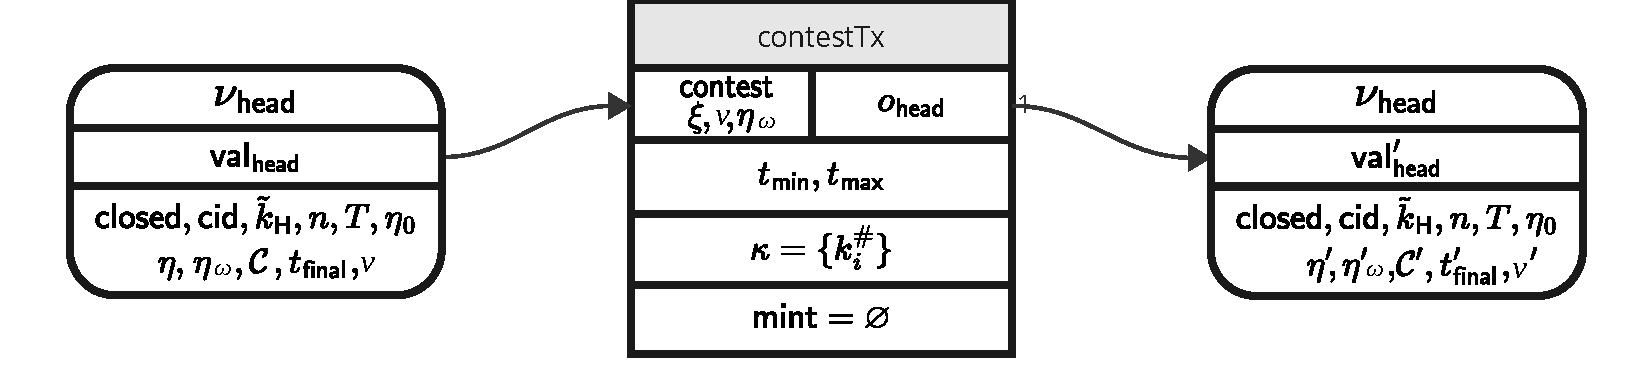
\includegraphics[width=0.8\textwidth]{figures/contestTx.pdf}
	\caption{\mtxContest{} transaction spending the $\stClosed$ head output and
		producing a different $\stClosed$ head output.}\label{fig:contestTx}
\end{figure}

\noindent The state-machine validator $\nuHead$ is spent with
$\redeemerHead = (\mathsf{contest}, \mathsf{ContestType})$, where
$\mathsf{ContestType}$ is a hint how to verify the snapshot and checks:
\begin{menumerate}
	\item State is advanced from $\datumHead \sim \stOpen$ to
	$\datumHead' \sim \stClosed$, parameters $\cid,\hydraKeys,\cPer$
	stay unchanged and the new state is governed again by $\nuHead$
	\[
		(\stClosed,\cid,\hydraKeys,\cPer,v,s,\eta,\eta_{\Delta},\contesters,\Tfinal) \xrightarrow[\mathsf{ContestType}]{\stContest} (\stClosed,\cid,\hydraKeys,\cPer,v',s',\eta',\eta_{\Delta}',\contesters',\Tfinal')
	\]

	\item Last known open state version stays recorded in closed state
	\[
		v' = v
	\]

	\item Contested snapshot number $s'$ is higher than the currently stored snapshot number $s$
	\[
		s' > s
	\]

	\item Based on the redeemer $\mathsf{ContestType} = (\mathsf{Unused}, \xi) \cup (\mathsf{Used}, \xi,  \eta_{\omega})$, where $\xi$ is a multi-signature of the contesting snapshot and $\eta_{\omega}$ is a digest of the UTxO to decommit, two cases are distinguished:
	\begin{menumerate}
		\item $\mathsf{Unused}$: Contesting snapshot refers to the current state version $v$ and any UTxO to decommit need to be present in the closed state too.
		\[
			\msVfy(\hydraKeys,(\cid || v || s' || \eta' || \eta_{\Delta}'),\xi) = \true
		\]
		which implies $\eta_{\Delta}' = \eta_{\omega}$ while $\eta_{\omega}$ does not need to be provided.
		\item $\mathsf{Used}$: Contesting snapshot refers the previous state version $v - 1$ and any UTxO to decommit must not be recorded in the closed state.
		\[
			\eta_{\Delta}' = \bot
		\]
		\[
			\msVfy(\hydraKeys,(\cid || v - 1 || s' || \eta' || \eta_{\omega}),\xi) = \true
		\]
		where $\eta_{\omega}$ is provided by the redeemer\footnote{$\eta_{\omega}$ needs to be provided to verify the signature, but is otherwise not relevant for the closed state}.
	\end{menumerate}
	% TODO: detailed CDDL definition of msg

	\item The single signer $\{\keyHash\} = \txKeys$ has not already contested and is added to the set of contesters
	\[
		\keyHash \notin \contesters
	\]
	\[
		\contesters' = \contesters \cup \keyHash
	\]
	\item Transaction is posted before deadline
	\[
		\txValidityMax \leq \Tfinal
	\]
	\item Contestation deadline is updated correctly to
	\[
		\Tfinal' = \left\{\begin{array}{ll}
			\Tfinal     & \mathrm{if} ~ |\contesters'| = n, \\
			\Tfinal + T & \mathrm{otherwise.}
		\end{array}\right.
	\]
	\item Value in the head is preserved
	\[
		\valHead' = \valHead
	\]
	\item Transaction is signed by a participant
	\[
		\exists \{\cid \mapsto \keyHash_{i} \mapsto 1\} \in \valCommit{i} \Rightarrow \keyHash_{i} \in \txKeys
	\]
	\item No minting or burning
	\[
		\txMint = \varnothing
	\]
\end{menumerate}

\subsection{Fan-Out Transaction}

Once the contestation phase is over, a head may be finalized by posting a
\mtxFanout{} transaction (see Figure~\ref{fig:fanoutTx}), which
distributes UTxOs from the head according to the latest state. It consists of
\begin{itemize}
	\item one input spending from $\nuHead$ holding the $\st$, and
	\item outputs $o_{1} \dots o_{m+n}$ to distribute UTxOs.
\end{itemize}

Note that \mtxFanout{} represents a final transition of the state machine and
hence there is no state machine output.

\begin{figure}
	\centering
	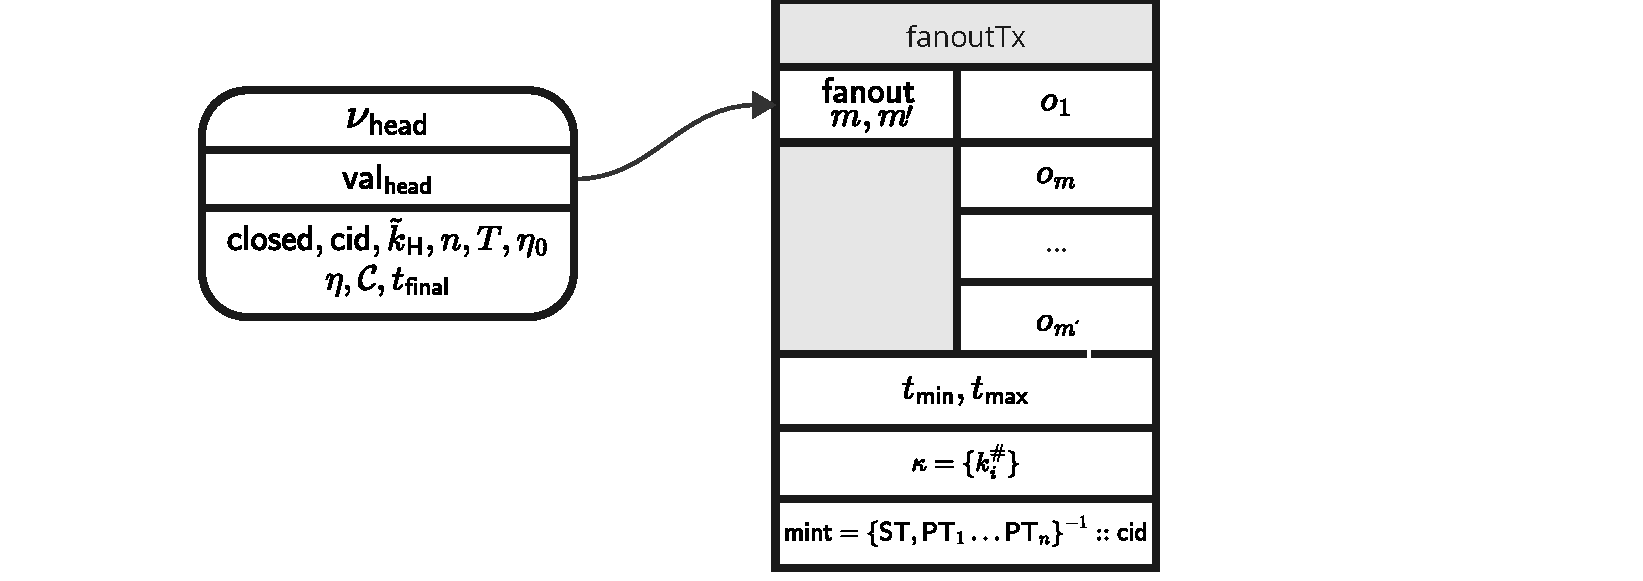
\includegraphics[width=0.8\textwidth]{figures/fanoutTx.pdf}
	\caption{\mtxFanout{} transaction spending the $\stClosed$ head output and
		distributing funds with outputs $o_{1} \dots o_{m}$.}\label{fig:fanoutTx}
\end{figure}

\noindent The state-machine validator $\nuHead$ is spent with
$\redeemerHead = (\mathsf{fanout}, m, n)$, where $m$ and $n$ are
outputs to distribute from the $\stClosed$ state, and checks:
\begin{menumerate}
	\item State is advanced from $\datumHead \sim \stClosed$ to terminal state
	$\stFinal$: % XXX: What does this actually mean?
	\[
		(\stClosed,\cid,\hydraKeys,\cPer,v, s,\eta,\eta_{\Delta},\contesters,\Tfinal) \xrightarrow[m,n]{\stFanout} \stFinal
	\]
	\item The first $m$ outputs are distributing funds according to $\eta$. That is,
	the outputs exactly correspond to the UTxO canonically combined $U^{\#}$ (see
	Section~\ref{sec:collect-tx}):
	\[
		\eta = U^{\#} = \hash(\bigoplus_{j=1}^{m} \bytes(o_{j}))
	\]
	\item The following $n$ outputs are distributing funds according to
	$\eta_{\Delta}$. That is, the outputs exactly correspond to the UTxO canonically
	combined $U^{\#}_{\Delta}$ (see Section~\ref{sec:collect-tx}):
	\[
		\eta_{\Delta} = U^{\#}_{\Delta} = \hash(\bigoplus_{j=m}^{m+n} \bytes(o_{j}))
	\]
	\item Transaction is posted after contestation deadline $\txValidityMin > \Tfinal$.
	\item All tokens are burnt
	$|\{\cid \mapsto \cdot \mapsto -1\} \in \txMint| = n + 1$.
\end{menumerate}

\noindent The $\muHead(\seed)$ minting policy governs the burning of tokens via
redeemer $\mathsf{burn}$ that:
\begin{menumerate}
	\item All tokens in $\txMint$ need to be of negative quantity
	$\forall \{\cid \mapsto \cdot \mapsto q\} \in \txMint : q < 0$.
\end{menumerate}

\FloatBarrier{}

%%% Local Variables:
%%% mode: latex
%%% TeX-master: "main"
%%% End:
